\documentclass{article}

\RequirePackage{tikz} % 绘图
\RequirePackage{pgf-umlcd} % 绘图:类图
\usetikzlibrary{positioning, shapes.geometric}

\begin{document}

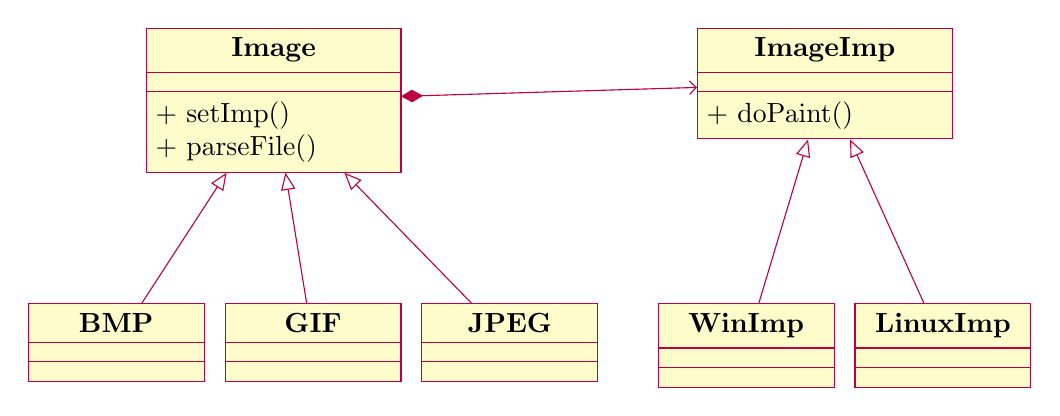
\begin{tikzpicture}
    \begin{class}[text width =3cm]{Image}{0 ,0}
        \attribute{}
		\operation{+ setImp() }	%公有成员
		\operation{+ parseFile() }                            %保护成员
        % \cdots
    \end{class}

	\begin{class}[text width=3cm]{ImageImp}{7,0}
        \attribute{}
		\operation{+ doPaint() }	
	\end{class}

    \begin{class}[text width=2cm]{BMP}{-2,-3.5}
        \inherit{Image}
    \end{class}

    \begin{class}[text width=2cm]{GIF}{0.5,-3.5}
        \inherit{Image}
    \end{class}

    \begin{class}[text width=2cm]{JPEG}{3,-3.5}
        \inherit{Image}
    \end{class}

    \begin{class}[text width=2cm]{WinImp}{6,-3.5}
        \inherit{ImageImp}
    \end{class}

    \begin{class}[text width=2cm]{LinuxImp}{8.5,-3.5}
        \inherit{ImageImp}
    \end{class}

    \composition{Image}{}{}{ImageImp}
\end{tikzpicture}

\end{document}